\section{Módulo de composición}
\label{sec:modcomp}

\torev{Última revisión realizada el 20-06-2012}

El módulo de composición es el encargado de crear un archivo de audio a partir de un archivo XML con información de figuras. Previo a crear el archivo de audio, será necesario componer la música en base a la configuración del usuario y a los datos de las figuras. La composición se verá plasmada en un fichero ABC siguiendo la notación musical ABC \color{blue}(Apéndice~\ref{sec:NotacionABC})\color{black}. De esta manera nos facilita la conversión en archivos de audio y además la posibilidad de mostrar la partitura de la pieza musical creada.

\color{blue}
Para la conversión y manipulación de los archivos de audio se usará los sistemas externos abcMIDI (Apéndice~\ref{sec:abcMIDI}) y Timidity (Apéndice~\ref{sec:Timidity}). abcMIDI se usará para convertir el archivo generado ABC en formato MIDI y a partir del MIDI se generará el formato WAV de sonido con Timidity. El proyecto de abcMIDI está formado por varios programas de los cuales sólo se utilizará abc2midi.
\color{black}

\subsection{Vista de Implementación}
La implementación realizada sigue el esquema de la Figura~\ref{fig:diagramaclasesMu}.\\

		\begin{figure}[!htbp]
		\centering
		\hspace*{0.0in}
		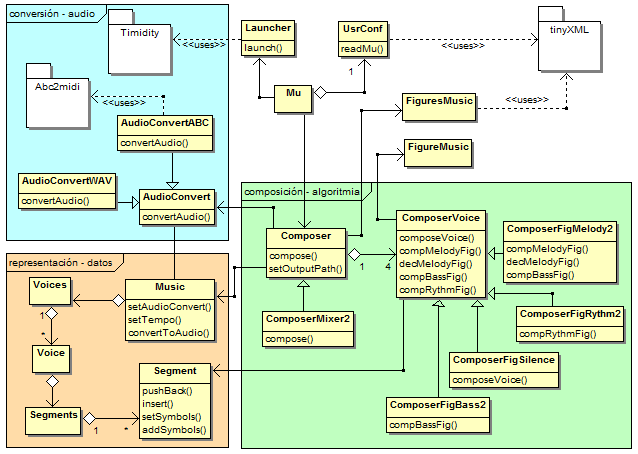
\includegraphics[scale=0.56]{graphics/diagramaclasesMU.png}
		\caption{Diagrama de clases del módulo de Composición}
		\label{fig:diagramaclasesMu}
		\end{figure}

Las clases más importante que podemos observar son:\\

\begin{itemize}

	\item \textbf{Mu:} se trata de la clase que controla la ejecución de este módulo. Se ocupa de crear y coordinar las clases principales de la composición. Además, al final se encarga de llamar al programa Timidity para que realice la conversión de Midi a Wav.
	
	\item \textbf{UsrConf:} como se explica en posteriores secciones, es una clase común que se ocupa de la lectura de los archivos de configuración que el usuario a especificado mediante la interfaz gráfica.
	
	\item \textbf{FiguresMusic:} es necesario crear una clase a partir de Figures que nos brinde una funcionalidad extra necesaria para el módulo de composición. Se explica más adelante los motivos de esta necesidad.
	
	\item \textbf{FigureMusic:} se trata de una extensión de la clase Figure, a la que toma como padre. Se explica más adelante los motivos de su creación.

	\item \textbf{Launcher:} ofrece la funcionalidad para ejecutar una aplicación externa. Se detalla más adelante, en la Sección~\ref{sec:arqMuphic}.

	\item \textbf{TinyXML:} Se trata de un paquete externo de código libre que permite generar y manipular archivos XML.

\end{itemize}

El resto de clases podemos separarlas en tres apartados diferentes según su objetivo principal:\\

Compositores - Algoritmia (color verde Figura~\ref{fig:diagramaclasesMu}):

\begin{itemize}
	
	\item \textbf{Composer:} encargado de procesar las figuras de entrada y crear la estructura de los datos de música. Su principal cometido es componer la música sirviendose de los métodos de composición que albergan los compositores de voces. Otra responsabilidad importante es crear el tipo de conversor adecuado para transformar nuestra notación musical en archivos de audio.

	\item \textbf{ComposerVoice:} la tarea principal de un compositor de voz es crear un segmento de música a partir de una figura de entrada. Existe la posibilidad de componer música para las cuatro diferentes voces identificadas (ver Sección~\ref{sec:algComposicion}). De esta clase extienden los diferentes algoritmos de composición implementados.

	\item \textbf{ComposerFigMelody2:} un ejemplo de clase que extiende de ComposerVoice que implementa la funcionalidad de crear música para las voces primera, segunda y tercera con los métodos compMelodyFig( ), decMelodyFig( ) y compBassFig( ).

	\item \textbf{ComposerFigBass2, ComposerFigRythm2:} se explican con mayor minuciosidad los algoritmos implementados en la Sección~\ref{sec:algComposicion}).

	\item \textbf{ComposerFigSilence:} clase encargada de crear una voz que esté en silencio. Esto ocurre cuando el usuario desactiva alguna de las voces de composición.

	\item \textbf{ComposerMixer2:} clase que hereda de Composer. Es una de las implementaciones realizadas que cumple con los cometidos de los que está encargado la clase padre.

\end{itemize}

Representación - Datos (color salmón Figura~\ref{fig:diagramaclasesMu}):

\begin{itemize}
	
	\item \textbf{Music:} encargado de almacenar la pieza musical que se está componiendo. Además debe comunicarse con AudioConvert para generar el archivo de audio. Esta clase se detalla con mayor detalle en la Sección~\ref{sec:repMusic}.

	\item \textbf{Voices, Voice, Segments:} Todas estas clases se detallan en la Sección~\ref{sec:repMusic}.

	\item \textbf{Segment:} es la unidad sobre la que trabajan los compositores de voces. Se usa como contenedor de las notas creadas por los diferentes algoritmos. Más información en la Sección~\ref{sec:repMusic}.

\end{itemize}

Conversión - Audio (color azul Figura~\ref{fig:diagramaclasesMu}):

\begin{itemize}
	
	\item \textbf{AudioConvert:} la principal función es convertir los datos que se manejan en los compositores dentro del sistema en un archivo de audio que permita reproducirse.

	\item \textbf{AudioConvertABC:} esta clase implementa una posible solución a la conversión entre nuestra notación musical y una salida estandar de audio. En este caso primero se transforma nuestra notación en un archivo con notación ABC y seguidamente se usa la aplicación externa Abc2midi para convertir el archivo ABC en un archivo de sonido Midi

	\item \textbf{AudioConvertWAV:} de forma experimental se desarrolló un sintetizador de sonido que, a partir de nuestra notación, generaba directamente un archivo wav sin compresión. Actualmente no se usa, ya que se obtienen con Abc2midi y Timidity archivos de sonido con mejor calidad y riqueza.

	\item \textbf{Abc2midi:} aplicación externa encargada de convertir un archivo de entrada con formato ABC en un archivo de sonido midi.

	\item \textbf{Timidity:} aplicación externa capaz de repoducir y convertir diferentes formatos de audio. En nuestro sistema se utiliza para convertir el archivo de sonido midi en wav.

\end{itemize}
	
El fujo de ejecución de una composición completa viene representado la Figura~\ref{fig:diagramaflujoMU1} y la Figura~\ref{fig:diagramaflujoMU2} con diagramas de secuencia o flujo. El primer diagrama reproduce la ejecución a alto nivel mientras que el segundo diagrama detalla la parte de ejecución encargada de la composición y conversión a archivo de sonido.

		\begin{figure}[!htbp]
		\centering
		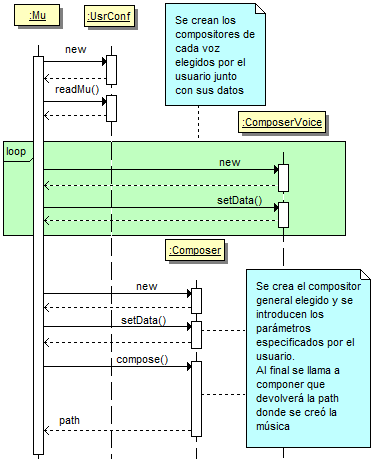
\includegraphics[scale=0.6]{graphics/diagramaflujoMU1.png}
		\caption{Flujo de ejecución alto nivel de abstracción del módulo de composición}
		\label{fig:diagramaflujoMU1}
		\end{figure}

		\begin{figure}[!htbp]
		\centering
		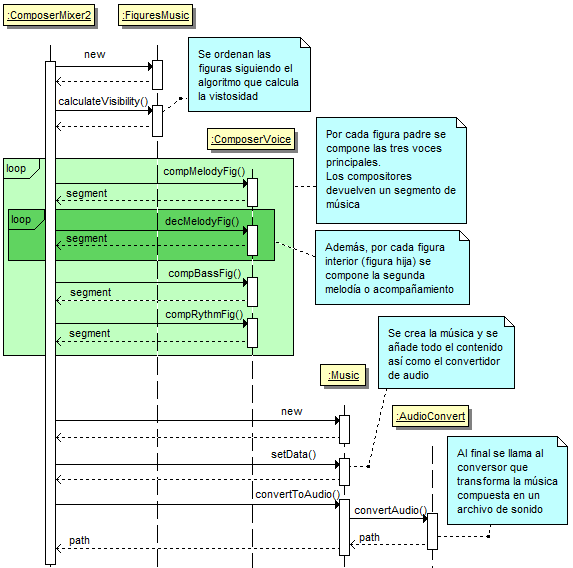
\includegraphics[scale=0.6]{graphics/diagramaflujoMU2.png}
		\caption{Dentro del módulo de composición, flujo de ejecución de los compositores}
		\label{fig:diagramaflujoMU2}
		\end{figure}



%--------------------------------------------------------------------------------------------------------------
\subsection{Figuras Musicales}

El módulo de composición trata las figuras según sus necesidades. Por ello, lo que necesita saber de cada figura además de todos los datos que se encuentran dentro de Figures es la relevancia o vistosidad de cada una, para ello hereda de las clases Figures y Figure mencionadas anteriormente en la Sección~\ref{subsec:usosFigure}, con las clases nuevas llamadas FiguresMusic y FigureMusic (Figura~\ref{fig:diagramaClasesFigureMusic}).

		\begin{figure}[!htbp]
		\centering
		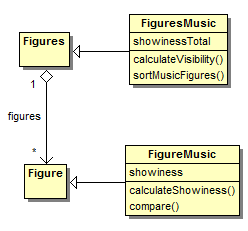
\includegraphics[scale=0.6]{graphics/diagramaClasesFigureMusic.png}
		\caption{Diagrama de las clases Figures y FiguresMusic}
		\label{fig:diagramaClasesFigureMusic}
		\end{figure}

A la clase FigureMusic se le añade la siguiente funcionalidad:

\begin{itemize}

	\item{calcularVistosidad}: Se calcula la relevancia de una figura dentro de una imagen con los siguientes valores: cantidad de rojo de la figura, cantidad de verde de la figura, cantidad de azul de la figura, área de la figura y distancia al centro de la imagen. Cada característica tiene su propio peso. La fórmula que relaciona todas estas características se ve con detalle en la Sección~\ref{sec:algComposicion}. Es necesario este valor para poder clasificar las figuras y así los compositores puedan usar las figuras de forma organizada.

	\item{compare}: Compara dos figuras según el valor de la vistosidad. Si dos figuras tienen misma vistosidad entonces tienen misma relevancia dentro de la imagen. Se emplea para poder ordenar las figuras.

\end{itemize}

A FiguresMusic se le añaden los elementos necesarios para poder considerar y utilizar la nueva funcionalidad añadida a FigureMusic:

\begin{itemize}

	\item{calcuteVisibility}: Primero calcula la vistosidad de cada figura si es que no se ha calculado ya, tomando los valores. Después se normalizan esos valores teniendo en cuenta el total de todas las figuras y la media. Función que usa sortMusicFigures para poder después ordenar las figuras.

	\item{sortMusicFigures}: Dada una lista de figuras, devuelve la lista ordenada según la vistosidad de las figuras. Esta funcionalidad se utiliza por parte de los compositores, para ordenar las figuras por su criterio de relevancia dentro de la imagen.

\end{itemize}